    \documentclass[conference]{IEEEtran}
\IEEEoverridecommandlockouts
% The preceding line is only needed to identify funding in the first footnote. If that is unneeded, please comment it out.
\usepackage{cite}
\usepackage{amsmath,amssymb,amsfonts}
\usepackage{algorithmic}
\usepackage{graphicx}
\usepackage{textcomp}
\usepackage{xcolor}
\def\BibTeX{{\rm B\kern-.05em{\sc i\kern-.025em b}\kern-.08em
    T\kern-.1667em\lower.7ex\hbox{E}\kern-.125emX}}
\begin{document}



\title{Predicting Hard Drive Failures using Machine Learning\\}



\author{
\IEEEauthorblockN{Asanga Ramanayaka}
\IEEEauthorblockA{\textit{Department of Computer Science} \\
\textit{Bowling Green State University}\\
Bowling Green, Ohio \\
asangar@bgsu.edu}
\and

\IEEEauthorblockN{Gamage Upeksha Maduwanthi Perera}
\IEEEauthorblockA{\textit{Department of Computer Science} \\
\textit{Bowling Green State University}\\
Bowling Green, Ohio \\
gperera@bgsu.edu}
\and

\IEEEauthorblockN{Shadi Moradi}
\IEEEauthorblockA{\textit{Department of Computer Science} \\
\textit{Bowling Green State University}\\
Bowling Green, Ohio \\
smoradi@bgsu.edu}
\and

\IEEEauthorblockN{Venkata SaiRam Sampath Yelchuri}
\IEEEauthorblockA{\textit{Department of Computer Science} \\
\textit{Bowling Green State University}\\
Bowling Green, Ohio \\
yvenkat@bgsu.edu}
\and

\IEEEauthorblockN{Robert Green}
\IEEEauthorblockA{\textit{Department of Computer Science} \\
\textit{Bowling Green State University}\\
Bowling Green, Ohio \\
greenr@bgsu.edu}
}

\maketitle

\begin{abstract}
Failing a hard drive can be costly. In this study, the main goal is to predict hard drive failures of various hard drive manufacturers accurately using machine learning techniques. This research applies two widely used machine learning approaches like Decision Tree Classifier and Random Forest Classifier on the Backblaze data-set. This study also provides an overview of different feature selection techniques like Recursive Feature Selection (RFE) or Model based Feature Selection. These methods have revealed some promising results with accuracy more than 80\%. At the same time, this study outperformed some previous studies by predicting hard drive failures based on splitting the data-set by hard drive manufactures.\\
\end{abstract}



\begin{IEEEkeywords}
Hard drive failure prediction, SMART Attributes, Machine Learning, Decision Tree, Random Forest, Recursive Feature Elimination, Receiver Operating Characteristic curve
\end{IEEEkeywords}

\section{Introduction}
In the modern world, people are producing a massive amount of data. To store this data, different kinds of storage devices are used, but still, hard drives are the most commonly used storage devices in the world. The most important feature of a storage device is the reliability. Usually, hard disk drives are considered to be durable and reliable, however recent studies has shown that hard drive is the most frequently replaced device in data centers \cite{b1}. 
Hard drive failure can be extremely costly for any company or any user because it can lead to an irreplaceable data loss or a live server crash which can cost millions of dollars damage \cite{b2}. Therefore, it is important to predict hard drive failures in advance. Most of the hard drive manufacturing companies have integrated advanced technologies such as Self-Monitoring, Analysis and Reporting Technology (SMART) to notify users any possibility of hard drive failures \cite{b3}. SMART attributes contain several numerical values which represent the current condition of the hard drive such as read error rate, seek error rate, spin up time, temperature, power on hours, relocated sectors count etc. \cite{b4,b5}. By analyzing the changes of these attributes, hard drive failure predictions have been made by previous researchers.\\ 


The main goal of this research is to improve the prediction accuracy by analyzing SMART attributes of hard drives separately for each hard drive manufacturer using machine learning techniques. The layout of this paper is as follows. Related studies published by previous researchers, is discussed in the section II. Information on Backblaze dataset, on which this research was performed, is included in the section III. The methodology section contain the experimental analysis and the methods used in this study. Comparisons of the outputs which were generated in the analysis and the threats to validity are investigated in the results and discussion section. Finally, we present our findings and the potential future developments in the conclusion.

\section{Background}

There are several studies which used machine learning and statistical methods to improve hard drive failure prediction. Most of the research uses SMART attributes for the prediction \cite{b2,b3,b4} while others use failure logs and captured disk events  \cite{b6,b7}. All those studies calculate failure prediction accuracy rate and false alarm rate (FAR). In general, failure prediction rate varies between 20\%-60\% while FAR is around 0\%-3\%.
Murray and Hughes performed several studies on hard drive failure prediction. In their study \cite{b3} they introduced improved algorithms to implement in SMART attributes to increase correct prediction accuracy of hard drives. The prediction rate achieved in that study is 40\% and the FAR is 0.2\% \cite{b3}. Then, Murray and Hughes came up with non-parametric statistical methods to generate more accurate results with FAR 0.1\% \cite{b8}. Later, they were able to achieve more than 50\% prediction rate with FAR 0\%, using support vector machine (SVM) classifier \cite{b9}. Since then, prediction rates were improved stably by several other researchers.\\

Some researchers used different statistical techniques such as time series, maximum likelihood, Bayes classifiers, regression trees and evaluation matrices for predicting hard drive failures \cite{b4,b6,b10}. In addition to that, machine learning techniques such as Support Vector machine (SVM), Artificial Neural Networks (ANN), Classification Trees (CT) etc. were used in the studies \cite{b2,b4}. Zhu et al. used Backpropagation Artificial Neural Networks (BP ANN) and advanced SVM model with a dataset of more than 23000 hard disk drives to predict drive failures. They were able to achieve a failure detection rate of 95\% with a FAR 0.03\% which is a very high accuracy \cite{b4}.\\

Instead of using SMART attributes, Agarwal et al. tried to predict hard drive failures using checksum mismatch of disks. They used a rule-based classifier to attain 70\% accuracy \cite{b6}. In addition to that, Schroeder and Gibson predicted using mean-time-to-failure (MTTF) values \cite{b7}. On the other hand, Pang et al. discussed predicting actual failure time of hard disks \cite{b2}. They used Combined Bayesian Network (CBN) on SMART attributes to predict actual failure time 70\% accurately. In this study, four classifiers were trained by Back-propagation Artificial Neural Networks, Evolutionary Neural Network (ENN), Support Vector Machine (SVM) and Classification Trees (CT) \cite{b2}.\\

Yang and Hu changed the direction of hard drive failure prediction researches by using bigdata to train their machine learning model \cite{b10}. In this study, the researchers focused more on improving the quality of training the existing model, instead of building new advanced models. They used 74.5 million hard disk records to train their model Hdoctor and achieved about 98\% detection rate with a FAR of 0.3\% which is the best rate from all the previous studies \cite{b10}. In addition to that, Yang and Hu et al. emphasized how to improve the accuracy integrating bigdata. However, none of the studies predicted hard disk drive failures based on the manufacturer. In this paper, machine learning techniques were applied on the Backblaze dataset by splitting it into four datasets such as 'Seagate', 'Hitachi', 'Western Digital', and 'Toshiba'.\\



\section{Dataset}

Backblaze is a company which provides cloud data storage services for the users all over the world. They have published hard drive related data of their data centers on their website with free access. Backblaze dataset contains millions of records of hard drive data from 2013 to 2019.  \cite{b15}. By each year, more hard disks are added to the datacenter. From 2013 to 2019, there is a single record for each working hard drive for every day. Hence, this dataset can be considered as a relatively big dataset, therefore data from 2017 first quarter (1st of January to 31st of March) were used in this study to predict hard disk drive failures.\\

Backblaze dataset contains a set of CSV files. A single file contains information of all working hard drives at each day. There are many columns (85 + columns) available in each file such as serial number, model, capacity, failure status, and SMART (Self-Monitoring, Analysis and Reporting Technology) attributes \cite{b16}. SMART attributes are a set of flags as raw values. They represent the current condition of the hard drive \cite{b4}. Many of the SMART attribute fields are empty because most drives do not report values for all fields daily. However, Yang et al identified 22 basic SMART attributes which are meaningful, and Zhu et al. mentioned 10 SMART attributes in their paper which are useful for predicting hard drive failures as shown in Table I \cite{b4,b10}.\\

Any dataset can be categorized as one of structured, semi-structured or unstructured data. Dataset used in this study (Backblaze dataset) were identified as semi-structured data because number of fields changed from year to year. For instance, in 2015, five additional SMART attributes were added to the dataset, which means ten new columns were generated to store new values. Another example for semi structured nature of this dataset is the inconsistency of the fields. Some of the SMART attributes depend on the model of the hard drive and the manufacture. Backblaze dataset has several models of hard drives such as Seagate, Hitachi, Western Digital, Toshiba. Therefore, some of the fields are highly inconsistent and cannot be used in the analysis in the previous studies\cite{b15}. At the same time, the set of columns SMART values are stored are changed based on the manufacturer. Hence, In this study we split 2017 first quarter dataset into four based on manufacturer and ran predictive analysis on each dataset separately.\\

Failure of a hard drive defined in several ways in Backblaze dataset. Generally, it is identified as failed when a hard drive stops spin up or when it does not connect to the operating system. However, there are several other situations where it is considered to be failed. When the SMART stats show values that the number of bad sectors higher than a particular threshold value, existing hard drive is replaced by a new drive \cite{b7}.

\section{Methodology}

Variable selection or feature selection has become one of the much discussed topics in the research. Extraction the most significant set of variables is of major concern. The idea is to isolating the related features from a set of features and removing the features which has the least contribution to the target variable in order to achieve better accuracy for our model. The literature identifies several variables that are important for hard drive failures \cite{b17}. The identified nine raw SMART parameters number 5, 12, 187, 188, 189, 190, 198, 199 and 200. In this study we used several feature selection methods and compared the results with the literature.\\

  \begin{table}[hbt]
    \begin{center}
    \caption{Hard Drive Statistics}
    \begin{tabular}{||l|r|r|r|r||}
    \hline
    \textbf{Manufacturer} & \textbf{No. of Records} & \textbf{Failed drives} & \textbf{Failure \%} \\ \hline
    Toshiba     & 33,793  & 6   & 0.0178\%    \\ \hline    
    Western Digital     & 183,671  & 8   & 0.0044\%        \\ \hline
    Hitachi (HGST)     & 2,316,371  & 58   & 0.0025\%     \\ \hline
    Seagate     & 4,098,269  & 313   & 0.0076\%        \\ \hline
    
    \end{tabular}
    \end{center}
    \end{table}

First Backblaze 2017 Q1 dateset was split based on the manufacturer. There are four different manufacturers in the dataset. More than 60\% of the records are from Seagate hard drives. Rest of the hard drive types are Hitachi, Western Digital, and Toshiba. Table 1 represent the number of records and failures for each hard drive manufacturers. Furthermore, it indicates that the number of failed hard drives are extremely low when compared with the working hard drives which means this dataset is highly imbalanced. When analysing the these imbalanced datasets, we applied SMOTE (Synthetic Minority Over Sampling Technique) as a re-sampling techniques to generate synthetic data to improve the accuracy of the predictive analysis.



\subsection{Correlation Matrix with Heatmap}

Correlation positions how the features are associated to each other or the response variable. A Heatmap is used to detect which features are most related to the target variable, and each other. Python provides the seaborn library to plot the heatmap of correlated features.\\

{Pearson Correlation Coefficient:}
\\

\begin{equation}
    \centering
    \verb|R(X,Y)| = \frac{Cov(X,Y)}{(Var(X) * Var(Y))^\frac{1}{2}}
\end{equation}
\\

Where, Cov denote the covariance and Var denotes the variance.

\subsection{Recursive Feature Elimination (RFE)}

The Recursive Feature Elimination method is a recursive process that ranks features according to some degree of their importance. At each iteration, importance is calculated and the less significant feature is removed. (Granitto, Furlanello, Biasioli, \& Gasperi, 2006). According to literature, the recursion is necessary since the relative significance of each feature can variate considerably when estimated over a different subset of features through the stepwise elimination process. To calculate a final ranking the (inverse) order in which features are excluded is used. \\ 

Feature selection should be done in concurrence with the cross validation. For each fold, the dataset is split into train and test. Then the feature selection is done, and selected features are recorded. The model is tested, and final output is recorded. The output is set of votes and best set of features are selected based on the votes.\\


\subsection{Synthetic Minority Over Sampling Technique (SMOTE)}
A dataset is imbalanced if the classes are not approximately equally represented. In general, real-world data sets are mainly composed of ``normal'' cases with only a small proportion of ``abnormal'' or ``interesting'' samples. In addition, the cost associated with misclassifying an abnormal case as a normal sample is often much higher than the cost of the reverse error (Chawla, Bowyer, Hall, \& Kegelmeyer, 2002). Synthetic Majority Oversampling Technique (SMOTE) works by producing artificial examples from the class with lower number of cases. It produces cases along the line segments joining randomly chosen Q minority class cases and their k-nearest minority neighbors (Santo, Soare, Abreu, Ara´ujo, \& Santos, 2018). Number of failures in the BlackBaze dataset is significantly smaller, therefore SMOTE should be used. SMOTE should be done in concurrence with the cross validation correspondingly.

\section{Results And Discussions}

The literature suggests several variables that are important for hard drive failures \cite{b13}. With this scheme, we consider those nine raw SMART parameters number 5, 12, 187, 188, 189, 190, 198, 199 and 200 and compared those features for four different datasets.

\subsection{Feature Selection for Four Datasets}
We applied feature selection methods for Hitachi, Seagate, Toshiba and Western Digital. The primary feature selection method we considered was correlation plot where highly correlated variables were disregarded. 
\\

\begin{itemize}

    \item \textit{Feature Selection for Hitachi :}\\
    Hitachi consists of 2316371 hard drives and 23 variables. Number of distinct disks 32257 and number of failed disks is 58, which is extremely small number. Clearly we deal with unbalanced dataset.According to the correlation analysis for the Hitachi dataset (Table 1) 'smart 8', 'smart 12', 'smart 193', 'smart 196' are dropped.\\
    
    
    \begin{figure}[htbp]
        \centerline{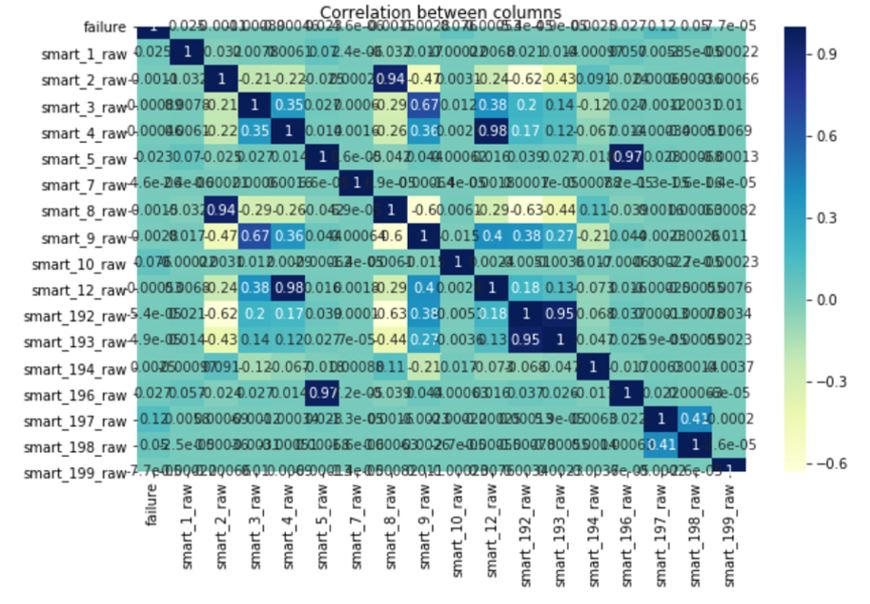
\includegraphics[width = 8cm]{Upeksha/Capture3.JPG}}
        \caption{Correlation Plot for Hitachi}
        \label{fig}
    \end{figure}

    \item \textit{Feature Selection for Western Digital :}\\
    Western Digital includes of 183671 hard drives and 22 attributes. The Number of distinct disks are 2285 and number of failed disks is 8, which is extremely small number. Clearly we deal with a highly imbalanced dataset. According to the correlation analysis for the Western Digital dataset fortunately, there are no features that were highly co-related except 'smart\_4\_raw' and 'smart\_192\_raw' which had 74 percent co-relation as shown in the below figure 2.\\
    
    
    \begin{figure}[htbp]
        \centerline{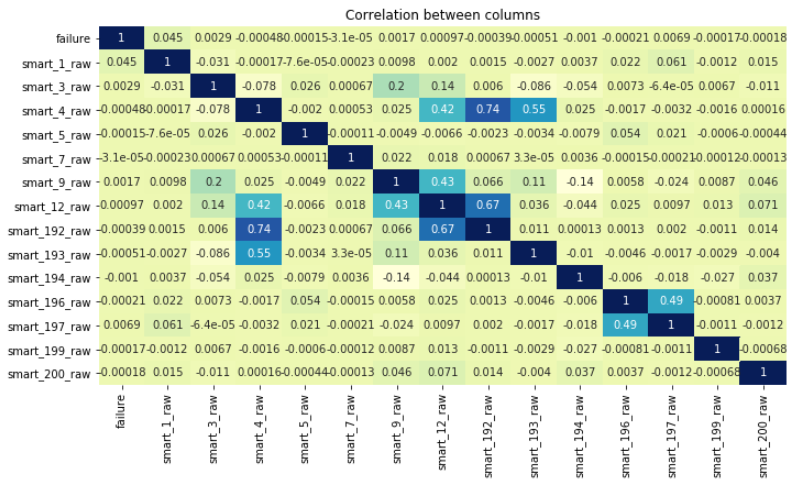
\includegraphics[width = 8cm]{Sampath/corelation_WD.PNG}}
        \caption{Correlation Plot for Western Digital}
        \label{fig}
    \end{figure}
    
    
    
    
    \item \textit{Feature Selection for Seagate :}\\
       Based on the previous research, raw SMART parameters number 5, 12, 187, 188, 189, 190, 198, and 199 were selected to run the analysis. Seagate is the biggest dataset from all four which consists of 4,098,269 records, however with only 313 failed hard drives. According to the correlation analysis smart variables 10, 192, 194, 197, and 199 were dropped due to higher correlation coefficients grater than 0.8.\\
       
        \begin{figure}[htbp]
        \centerline{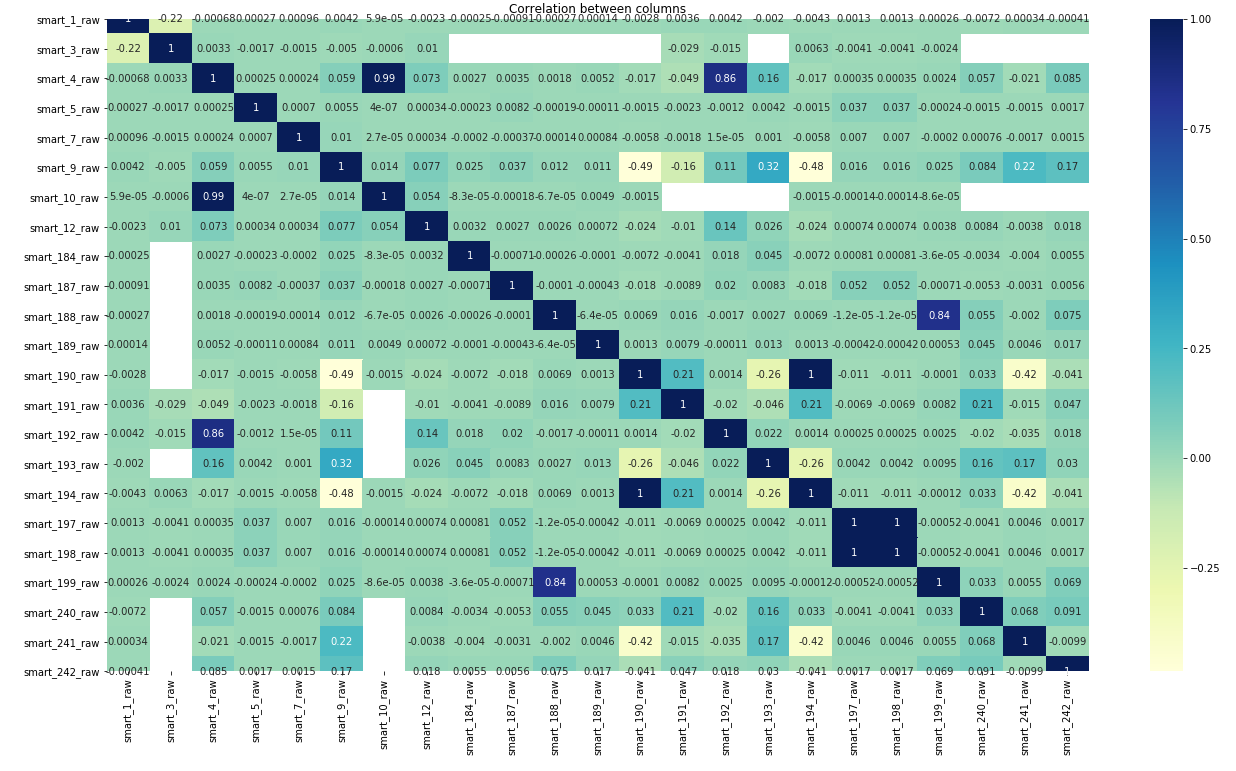
\includegraphics[width = 8cm]{Asanga/sgt_corr.PNG}}
        \caption{Correlation Plot for Seagate}
        \label{fig}
    \end{figure}
   

 
    
    
    \item \textit{Feature Selection for Toshiba :}\\
    Toshiba hard drive dataset consists of 33793 hard drives and 24 variables. Number of failed hard drives is 6, which is extremely small number compared to the dimension of the data. This shows that we are dealing with a highly sparse dataset. To reduce the dimension of the dataset first by doing some basic statistics like percentile, mean, std, etc, we are able to drop the following features: smart 1, 2, 7, 8, 10, 198, 220, 223,224, 240. Furthermore, according to the correlation between features, smart 9, 12, 196, 222 are dropped.
    
     \begin{figure}[htbp]
        \centerline{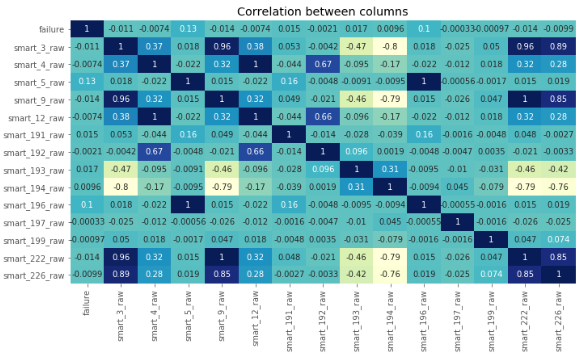
\includegraphics[width = 8cm]{Shadi/corr.PNG}}
        \caption{Correlation Plot for Toshiba}
        \label{fig}
    \end{figure}
    
\end{itemize}

\subsection{Recursive Feature Elimination for Four Datasets}

Recursive feature elimination was used with five fold cross validation. The feature selection should be done in conjunction with cross validation. For each fold, training and testing data are selected and feature selection is performed. Then the selected set of variables are utilized in the model and the results are recorded. Best set of features are selected from resulting votes. 

\begin{itemize}

    \item \textit{Recursive Feature Selection for Hitachi :}\\
    From the set of variables given in the literature \cite{b13} only 'smart 12', 'smart 5', 'smart 198', 'smart 199' are in the Hitachi data set. These variables can be compared with the highest ranking variables after recursive feature elimination output in table 1. Smart 5 has become the fifth highest ranking variable from the recursive feature elimination. The variables 199 and 198 are third and second lowest ranking variables. Also, smart 12 was dropped after the correlation analysis. It can be clearly seen that the list of variables from the recursive feature elimination output have complementary results compared to the literature.\\ 
    \begin{table}[h]
    \caption{Ranking of Features based on votes for Hitachi}
    \label{table_example}
    \begin{center}
    \begin{tabular}{|c||c|}
    \hline
    \textbf{Ranking} & \textbf{Features}\\ \hline
    1 & smart\_9\_raw\\\hline
    1 & smart\_194\_raw\\\hline
    1 & smart\_197\_raw\\\hline
    1.4 & smart\_5\_raw\\\hline
    2.2 & smart\_3\_raw\\\hline
    2.2 & smart\_4\_raw\\\hline
    3.2 & smart\_2\_raw\\\hline
    3.4 & smart\_192\_raw\\\hline
    5.4 & smart\_10\_raw\\\hline
    5.6 & smart\_1\_raw\\\hline
    5.6 & smart\_199\_raw\\\hline
    8 & smart\_198\_raw\\\hline
    9 & smart\_7\_raw\\\hline
    \end{tabular}
    \end{center}
    \end{table}

    \item \textit{Recursive Feature Selection for Western Digital :}\\
    From the set of variables given in the literature \cite{b13} only 'smart 5', 'smart 12', 'smart 198', 'smart 199', and 'smart 200', are present in the Western Digital data set. These variables can be compared with the highest ranking variables after recursive feature elimination output in table 2 as given below. Smart 5 has become the fifth highest ranking variable from the recursive feature elimination. The variables 7 and 4 are third and second lowest ranking variables. Also, smart 10, smart 11, and smart 198  were dropped after looking into the descriptive analysis. It can be clearly seen that the list of variables from the recursive feature elimination output have complementary results compared to the literature.\\
    
    \begin{table}[]
    \begin{center}
    \caption{Ranking of Features based on votes for Western Digital}
    \begin{tabular}{|c||c|}
    \hline
    \textbf{Ranking} & \textbf{Features}\\ \hline
    1.0     & smart\_1\_raw   \\ \hline
    1.0     & smart\_193\_raw \\ \hline
    1.0     & smart\_194\_raw \\ \hline
    1.2     & smart\_12\_raw  \\ \hline
    2.2     & smart\_3\_raw   \\ \hline
    2.6     & smart\_192\_raw \\ \hline
    3.4     & smart\_197\_raw \\ \hline
    3.6     & smart\_200\_raw \\ \hline
    4.2     & smart\_199\_raw \\ \hline
    6.6     & smart\_9\_raw   \\ \hline
    6.6     & smart\_196\_raw \\ \hline
    7.4     & smart\_4\_raw   \\ \hline
    8.6     & smart\_7\_raw   \\ \hline
    9.6     & smart\_5\_raw   \\ \hline
    \end{tabular}
    \end{center}
    \end{table}
    
    \item \textit{Recursive Feature Selection for Seagate :}\\
Table IV represents the rankings of the columns after running the recursive feature elimination for Seagate dataset. Top eight smart variables were selected from this table to run the analysis, in order to compare the results with literature based analysis. (smart 187, 198, 9, 193, 191, 190, 242, and 241) \\
    

 \begin{table}[hbt]
    \begin{center}
    \caption{Ranking of Features based on votes for Seagate}
    \begin{tabular}{|c||c||}
    \hline
    \textbf{Ranking} & \textbf{Features}\\ \hline
    1.0     & smart\_187\_raw   \\ \hline
    1.0     & smart\_198\_raw \\ \hline
    1.4     & smart\_9\_raw \\ \hline
    3.2     & smart\_193\_raw  \\ \hline
    3.4     & smart\_191\_raw   \\ \hline
    3.4     & smart\_190\_raw \\ \hline
    3.4     & smart\_242\_raw \\ \hline
    3.6     & smart\_241\_raw \\ \hline
    4.0     & smart\_240\_raw \\ \hline
    4.2     & smart\_5\_raw   \\ \hline
    7.0     & smart\_189\_raw \\ \hline
    8.2     & smart\_184\_raw   \\ \hline
    9.4     & smart\_4\_raw   \\ \hline
    9.6     & smart\_1\_raw   \\ \hline
    10.2     & smart\_12\_raw \\ \hline
    10.6     & smart\_188\_raw   \\ \hline
    11.4     & smart\_7\_raw   \\ \hline
    14.0     & smart\_3\_raw   \\ \hline
    \end{tabular}
    \end{center}
    \end{table}    
    
    
       \begin{table}[]
   \begin{center}
    \caption{Classification report for RFE output for Seagate}   
    \begin{tabular}{||l|l|l|l|l||}
    \hline
    Field & Classifier Accuracy & Precision & Recall & F1 Score \\ \hline
    1     & 0.99                & 1.00         & 0.99   & 1.00     \\ \hline
    2     & 0.99                & 1.00         & 0.99   & 1.00     \\ \hline
    3     & 0.99                & 1.00         & 0.99   & 1.00     \\ \hline
    4     & 0.99                & 1.00         & 0.99   & 1.00     \\ \hline
    5     & 0.99                & 1.00         & 0.99   & 1.00     \\ \hline
    \end{tabular}
    \end{center}
    \end{table}
    
    
    
    
    \item \textit{Recursive Feature Selection for Toshiba :}\\
    Recursive feature elimination is applied on the dataset along with different classifiers inside the k-fold cross-validation to select top 5 features, each of the classifiers selected different set of features. However, based on the accuracy and analysing confusion matrix for Toshiba hard drive Logistic regression with SMOTE oversampling technique the top selected features are as follows: smart 3, 5, 191, 192, and 226.\\
    
    \begin{table}[]
    \begin{center}
    \caption{Ranking of Features based on votes for Toshiba}
    \begin{tabular}{|c||c|}
    \hline
    \textbf{Ranking} & \textbf{Features}\\ \hline
    1.0     & smart\_3\_raw   \\ \hline
    1.0     & smart\_5\_raw \\ \hline
    1.0     & smart\_191\_raw \\ \hline
    1.0     & smart\_192\_raw  \\ \hline
    1.6     & smart\_226\_raw   \\ \hline
    2.4     & smart\_4\_raw \\ \hline
    3.4     & smart\_199\_raw \\ \hline
    3.8     & smart\_193\_raw \\ \hline
    4.4     & smart\_194\_raw   \\ \hline
    5.4     & smart\_197\_raw \\ \hline
    \end{tabular}
    \end{center}
    \end{table}
    
\end{itemize}

\subsection{Comparing Results of Predictive Models}
In this section, we will discuss and compare the results of all the four data sets with respect to the results that are generated using the features from the literature. Since, we have a data processing constraint, we try to apply Random Forest Classifier on the smaller data sets and Decision Tree Classifier for the larger data sets. 

\begin{itemize}
    
    \item \textit{Decision Tree Classifier for Hitachi :}\\
    The set of variables given in the \cite{b13} 2017 and the resultant variables from Recursive Feature Elimination (RFE) are used in a Decision Tree Classifier separately.\\
    
    \begin{table}[]
    \begin{center}
    \caption{Classification report for RFE output for Hitachi}
    \begin{tabular}{||l|l|l|l|l||}
    \hline
    Field & Classifier Accuracy & Precision & Recall & F1 Score \\ \hline
    1     & 0.98                & 1         & 0.99   & 0.99     \\ \hline
    2     & 0.99                & 1         & 0.99   & 1        \\ \hline
    3     & 0.98                & 1         & 0.99   & 0.99     \\ \hline
    4     & 0.99                & 1         & 0.99   & 1        \\ \hline
    5     & 0.97                & 1         & 0.98   & 0.99     \\ \hline
    \end{tabular}
    \end{center}
    \end{table}
    
    According to Table 3 as mentioned below, the decision tress classifier indicates ~ 0.99 accuracy. The set of variables given in the \cite{b13} produce an out put with same level of accuracy with decision tree classifier. 
    
    \begin{figure}[htp]
        \centering
        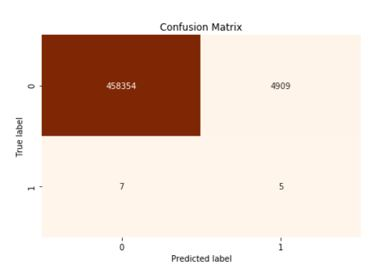
\includegraphics[width=8cm]{Upeksha/Capture6.JPG}
        \caption{Confusion Matrix of Decision Tree (RFE) for Hitachi}
    \end{figure}

    \begin{figure}[htp]
        \centering
        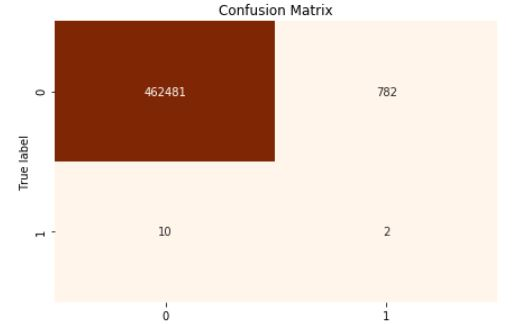
\includegraphics[width=8cm]{Upeksha/Capture7.JPG}
        \caption{Confusion Matrix of Decision Tree (Lit) for Hitachi}
    \end{figure}

    \item \textit{Random Forest Classifier for Western Digital :}\\
    The set of variables given in the \cite{b13} and the resultant variables from Recursive Feature Elimination (RFE) are used in a Random Forest Classifier separately.\\
    
   \begin{table}[]
   \begin{center}
    \caption{Classification report for RFE output for Western Digital}   
    \begin{tabular}{||l|l|l|l|l||}
    \hline
    Field & Classifier Accuracy & Precision & Recall & F1 Score \\ \hline
    1     & 0.83                & 1         & 0.83   & 0.91     \\ \hline
    2     & 0.83                & 1         & 0.83   & 0.91     \\ \hline
    3     & 0.83                & 1         & 0.84   & 0.91     \\ \hline
    4     & 0.83                & 1         & 0.83   & 0.91     \\ \hline
    5     & 0.83                & 1         & 0.84   & 0.91     \\ \hline
    \end{tabular}
    \end{center}
    \end{table}

    \begin{figure}[htp]
        \centering
        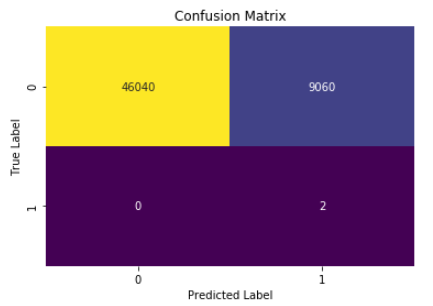
\includegraphics[width=8cm]{Sampath/confusion_Matrix.PNG}
        \caption{Confusion Matrix of Random Forest Classifier (RFE) for Western Digital}
    \end{figure}

    \begin{figure}[htp]
        \centering
        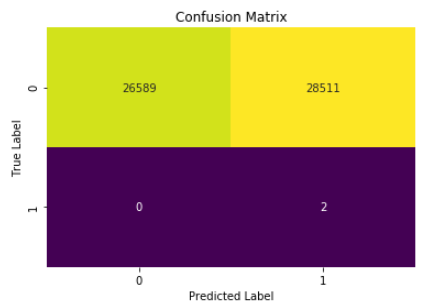
\includegraphics[width=8cm]{Sampath/confusion_Matrix_Lit.PNG}
        \caption{Confusion Matrix of Random Forest Classifier (Lit) for Western Digital}
    \end{figure}
    
    According to Table 4 as mentioned below, the Random Forest Classifier indicates ~ 0.83 accuracy. The set of variables given in the \cite{b13} produce an out put with less level of accuracy with Random Forest Classifier.\\ 
    
    
    \item \textit{Random Forest Classifier for Seagate :}\\
        Analysis was run using Random Forest Classifier for both RFE based and literature based scenarios. Resultant confusion matrices are shown in Figure 5 and 6 respectively. They indicate that in both cases the generated results are almost the same. Figure 11 and Figure 12 ROC curves generated for two analysis indicates same-like values for area under the curve (0.74 and 0.75). However, number of false alarms are higher in literature based analysis. On the other hand, both analysis has higher number of false negatives when compare to true positives. These missed alarms can be affected by the highly imbalanced nature of the dataset.\\
        
        
        \begin{figure}[htp]
        \centering
        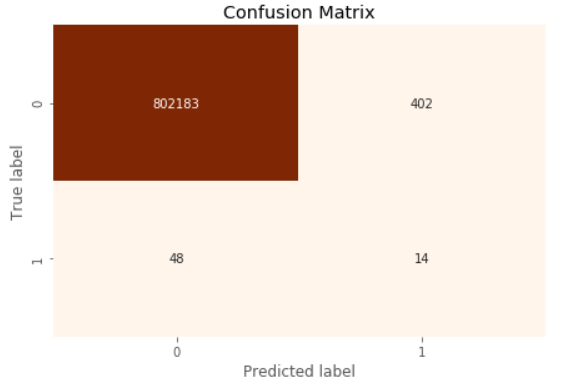
\includegraphics[width=8cm]{Asanga/sgt_cm_rfe.PNG}
        \caption{Confusion Matrix of Random Forest Classifier (RFE) for Seagate}
    \end{figure}
    
        \begin{figure}[htp]
        \centering
        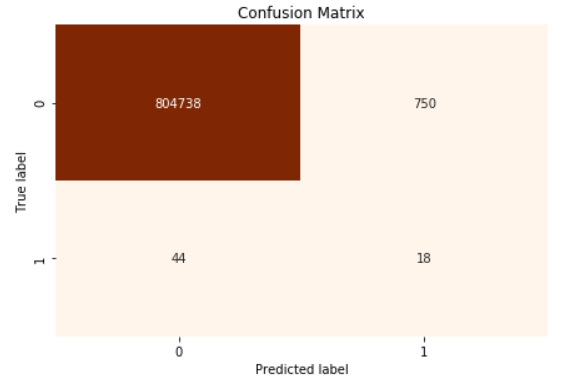
\includegraphics[width=8cm]{Asanga/sgt_cm_lit.PNG}
        \caption{Confusion Matrix of Random Forest Classifier (Lit) for Seagate}
    \end{figure}
    
            \begin{figure}[htp]
        \centering
        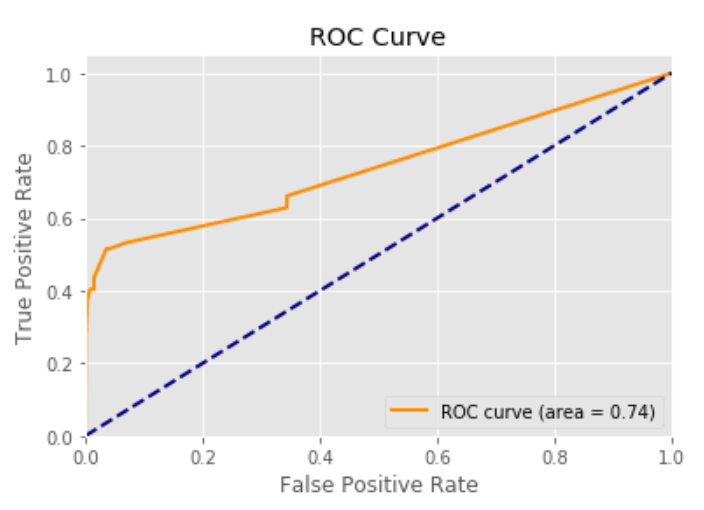
\includegraphics[width=8cm]{Asanga/sgt_roc_rfe.PNG}
        \caption{ROC Curve of Random Forest Classifier (RFE) for Seagate}
    \end{figure}
    
            \begin{figure}[htp]
        \centering
        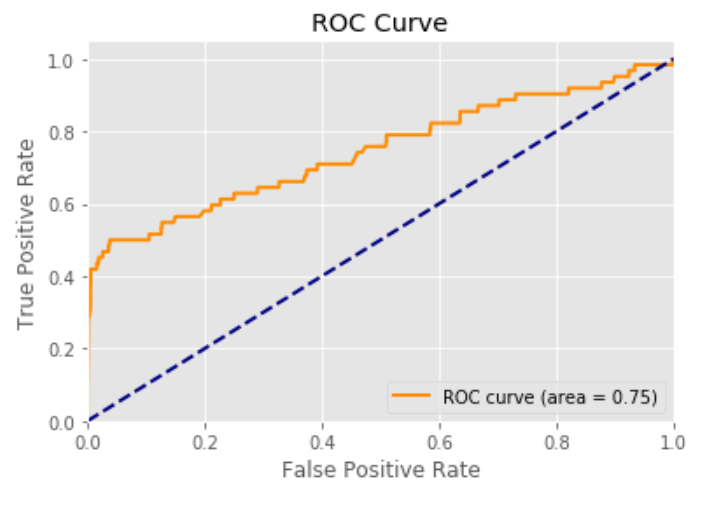
\includegraphics[width=8cm]{Asanga/sgt_roc_lit.PNG}
        \caption{ROC Curve of Random Forest Classifier (Lit) for Seagate}
    \end{figure}
    
    \item \textit{Random Forest Classifier for Toshiba :}\\
    The following classifiers and resampling techniques are applied on the data inside the k-fold cross-validation: Random Forest classifier with SMOTE oversampling which resulted in the accuracy of 0.7, F1-score of 0.44, and balanced accuracy of 0.55. Random Forest with ADASYN resampling technique that resulted in 0.78 accuracy. Decision Tree classifier with SMOTE method which resulted in 0.99 accuracy. Decision Tree classifier with ADASYN resampling which resulted in 0.99 accuracy. Finally, Logistic Regression with SMOTE oversampling that resulted in 78 percent accuracy. However, since the data is too sparse, considering and analysing confusion matrix it seems like for Toshiba dataset Logistic regression works the best to detect the failed hard drives. Logistic regression is able to detect both of the failed hard drives in the testing set with the fewest false alarm among other methods that is tried. After Logistic Regression, Random Forest classifier performed the best to detect the failures. 
    
       \begin{figure}[htbp]
        \centerline{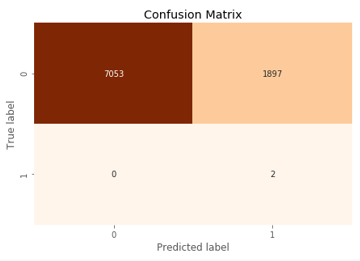
\includegraphics[width = 8cm]{Shadi/ConfusionMatrix.PNG}}
        \caption{Confusion Matrix Logistic Regression for Toshiba}
        \label{fig}
    \end{figure}
    
\end{itemize}


\section{CONCLUSION}

In this study, we compared results of two analysis; features selected by Recursive Feature Elimination (RFE) and by literature based selection for each datasets. For all the datasets, RFE based feature selection produced high accuracy than literature based selection. However, in the Seagate hard drive dataset, both methods produced equal results. The main reason for the higher accuracy of RFE based analysis can be the differences of datasets. Previous researchers have selected their features based on on year 2014 dateset. In our analysis we used 2017 Q1 dataset. On the other hand, most of the features remained same, however a few new columns were added to the dataset within this period. Furthermore, by splitting the dataset by manufacturer, we analyzed four datasets separately while the previous researchers analyzed all types of hard drives as a single dataset.

In addition to that, we identified that Random Forest Classifier works better than other binary classifiers for most of the datasets. However, for the Toshiba dataset Logistic Regression model performed slightly better. After trying several over-sampling techniques such as SMOTE, SVMSMOTE and ADASYN we determined SMOTE works fast and accurately than other two.


\begin{thebibliography}{99}

\bibitem{b1} K. V. Vishwanath and N. Nagappan, “Characterizing Cloud Computing Hardware Reliability,” in Proceedings of the 1st ACM Symposium on Cloud Computing, New York, NY, USA, 2010, pp. 193–204.
\bibitem{b2} S. Pang, Y. Jia, R. Stones, G. Wang, and X. Liu, “A combined Bayesian network method for predicting drive failure times from SMART attributes,” in 2016 International Joint Conference on Neural Networks (IJCNN), 2016, pp. 4850–4856.
\bibitem{b3} G. F. Hughes, J. F. Murray, K. Kreutz-Delgado, and C. Elkan, “Improved disk-drive failure warnings,” IEEE Trans. Reliab., vol. 51, no. 3, pp. 350–357, Sep. 2002.
\bibitem{b4} B. Zhu, G. Wang, X. Liu, D. Hu, S. Lin, and J. Ma, “Proactive drive failure prediction for large scale storage systems,” in 2013 IEEE 29th Symposium on Mass Storage Systems and Technologies (MSST 2013)(MSST), 2013, pp. 1–5.
\bibitem{b5} “Backblaze Hard Drive Stats.” [Online]. Available: https://www.backblaze.com/b2/hard-drive-test-data.html. [Accessed: 21-Oct-2018].


\bibitem{b6} V. Agrawal, C. Bhattacharyya, T. Niranjan, and S. Susarla, Prediction of Hard Drive Failures via Rule Discovery from AutoSupport Data. .
\bibitem{b7} B. Schroeder and G. A. Gibson, “Understanding Disk Failure Rates: What Does an MTTF of 1,000,000 Hours Mean to You?,” Trans Storage, vol. 3, no. 3, Oct. 2007.
\bibitem{b8}J. Murray, G. Hughes, and K. Kreutz-Delgado, “Hard drive failure prediction using non-parametric statistical methods,” Jan. 2003.
\bibitem{b9} J. F. Murray, G. F. Hughes, and K. Kreutz-Delgado, “Machine Learning Methods for Predicting Failures in Hard Drives: A Multiple-Instance Application,” J. Mach. Learn. Res., vol. 6, no. May, pp. 783–816, 2005.
\bibitem{b10} W. Yang, D. Hu, Y. Liu, S. Wang, and T. Jiang, “Hard Drive Failure Prediction Using Big Data,” in 2015 IEEE 34th Symposium on Reliable Distributed Systems Workshop (SRDSW), 2015, pp. 13–18.


\bibitem{b11} Chawla, N. V., Bowyer, K. W., Hall, L., \& Kegelmeyer, W. P. (2002). SMOTE: Synthetic Minority Over-sampling Technique. Journal of Artificial Intelligence Research.
\bibitem{b12} Granitto, P. M., Furlanello, C., Biasioli, F., \& Gasperi, F. (2006). Recursive feature elimination with random forest for PTR-MS analysis of. 
\bibitem{b13} Nicolas Aussel, S. J. (2017). Predictive models of hard drive failures based on operational data. IEEE Computer Society, Proceedings ICMLA 2017: 16th IEEE International Conference On Machine Learning And Applications, 619-625.
\bibitem{b14} Santo, M., Soare, J., Abreu, P., Ara´ujo, H., \& Santos, J. (2018). Cross-Validation for Imbalanced Datasets: Avoiding Overoptimistic and Overfitting Approache. IEEE Computational Intelligence Magazine .



\bibitem{b15} “Backblaze Drive Stats: 2018 Hard Drive Failure Rates,” Backblaze Blog | Cloud Storage & Cloud Backup, 16-Oct-2018. .
\bibitem{b16} “How Long Do Hard Drives Last: 2018 Hard Drives Stats,” Backblaze Blog | Cloud Storage & Cloud Backup, 01-May-2018. .
\bibitem{b17} “Backblaze Hard Drive Stats for 2017.” [Online]. Available: https://www.brighttalk.com/webcast/14807/300531/backblaze-hard-drive-stats-for-2017. [Accessed: 13-Nov-2018].
\bibitem{b18} “scikit-learn: machine learning in Python — scikit-learn 0.20.0 documentation.” [Online]. Available: https://scikit-learn.org/stable/. [Accessed: 13-Nov-2018].

 



\end{thebibliography}
\end{document}
